\documentclass{article}
\usepackage[colorlinks=true]{hyperref}
\usepackage{geometry}
\usepackage{fancyhdr}
\usepackage{palatino}
\usepackage{titlesec}
\usepackage{pbox}
\usepackage{multicol}
\usepackage{graphicx}
\usepackage{enumitem}

\renewcommand{\baselinestretch}{1.15}
\geometry{margin=1in}
\geometry{headheight=2in}
\geometry{top=2in}
\titlespacing\section{0pt}{12pt plus 2pt minus 2pt}{0pt plus 2pt minus 2pt}
\lhead{}
\rhead{}
\pagestyle{fancy}
\setlength{\parskip}{0.5em}
\date{\today}

\title{CS 145 Milestone 1 - ToMEto}
\author{Jonathan Joo, Matthew Jin, Boyu (Charlie) Tong, Albert Ge}
\chead{%
  {\vbox{%
      \vspace{2mm}
      \large
      Networks: Structure Economics \hfill
      Caltech CMS/CS/EE 145 \hfill \\[1pt]
      CS 145 Milestone 1 - ToMEto \hfill
      \date{\today} \\
    }
  }
}

\linespread{1.5}


\begin{document}
\maketitle

\section{Goals}
As per our project plan, the two early milestones we wanted to accomplish were:
\begin{enumerate}
    \item Begin data collecting
    \item Set up storate environments
\end{enumerate}

On the specifics of the milestones, these past two weeks we planned on familiarizing ourselves with the environment, i.e. 
looking at APIs, figuring out which websites to crawl. Additionally, as per last week's meeting, we set out to investigate
\begin{enumerate}
    \item More of the literature regarding recipe recommendations
    \item Existing recipe applications 
    \item Obtain data quickly, either by scraping ourselves or asking others 
\end{enumerate}

\section{Progress}
In light of the goals we set out to accomplish, here we describe our current progress.
\subsection{Literature}

Much of the existing literature uses machine-learning techniques to make 
recommendations, rate recipes, or make suggestions about substituting ingredients, and due to our limited knowledge
in this field, it is not a path we wish to pursue much further. Consequently, we refine our search for simpler
food-related papers. Before we decided on a use case, we perused through a variety of articles, some of which
we list and reflect on below: \\

\begin{enumerate}
    \item
    \textbf{Personalized recipe for healthy choices:} \texttt{http://dl.acm.org/citation.cfm?id=1943487} \\
    This describes a prototype for personalizing recipes such that the result returned to the user
    is nutritious and healthy. This allows the user to specify down to the nutrient level (e.g. vitamins and fibers),
    and takes information about the user's past meal choices 
    
    \textbf{Geography and Similarity of Regional Cuisines in China} \\
    \texttt{http://journals.plos.org/plosone/article?id=10.1371\%2Fjournal.pone.0079161}.
    This is a paper about
    
\end{enumerate}

\subsection{Use case} 
Because recipe suggestion appears to be largely based on machine-learning, we turned instead
our attention a use case that relies less on recommendations, and looks into how 
food is represented as a graph, and the connections between different ingredients. In particular,
we have currently decided to focus on utilizing \textit{fusion of cuisines}, given that
particular ingredients may be cross-utilized in different regions. Therefore, our use case is to:
\begin{enumerate}
    \item User inputs what fusion cuisine they desire 
    \item Result returns a recipe that is from one cuisine, but contains substituted ingredients that 
        exist in a second cuisine, thereby creating a fusion dish 
\end{enumerate}


\subsection{Data collection \& storage} 
We have begun acquiring data from online recipe sources, namely \texttt{http://cooking.nytimes.com} and \texttt{http://allrecipes.com} because their sites make it easy to extract the list of ingredients. We wrote scrapers that crawl the websites, collecting recipe webpages and saving them locally as html/text files. Right now we are downloading recipes at about 1000 per hour from each website. We employ a sleep timer to slow down downloads and avoid being throttled.

For parsing the data, we wrote scripts that employ regex that extract the ingredients from each recipe webpage. Right now the data is still stored locally in text files. In the upcoming week, we will work on postprocessing the ingredients list. One specific task that needs to be done is removing the quantifiers (1 cup, 1 tablespoon, etc.) from the \texttt{http://allrecipes.com} recipes. The \texttt{http://cooking.nytimes.com} recipes have quantifiers separate, so not much postprocessing needs to be done for them.


\subsection{Front-end APIs}
For front-end, we were able to get some baseline code up and running for our website. We currently have two pages, a landing page and then a page that allows you to enter up to ten ingredients. Upon pressing a button, these ingredients are then sent to app.py, which is a python script which will likely handle all of the algorithms with this information. The ingredients are conveniently stored in an array, so that our backend can use these inputs to determine which ingredients to generate. 

The following sites were useful in creating this website, which is fully interactive and usable right now.
\begin{itemize}
\item http://code.tutsplus.com/tutorials/creating-a-web-app-from-scratch-using-python-flask-and-mysql--cms-22972 
\item http://www.randomsnippets.com/2008/02/21/how-to-dynamically-add-form-elements-via-javascript/ 
\end{itemize}

Here is a screenshot of our landing page: \\
\begin{center}
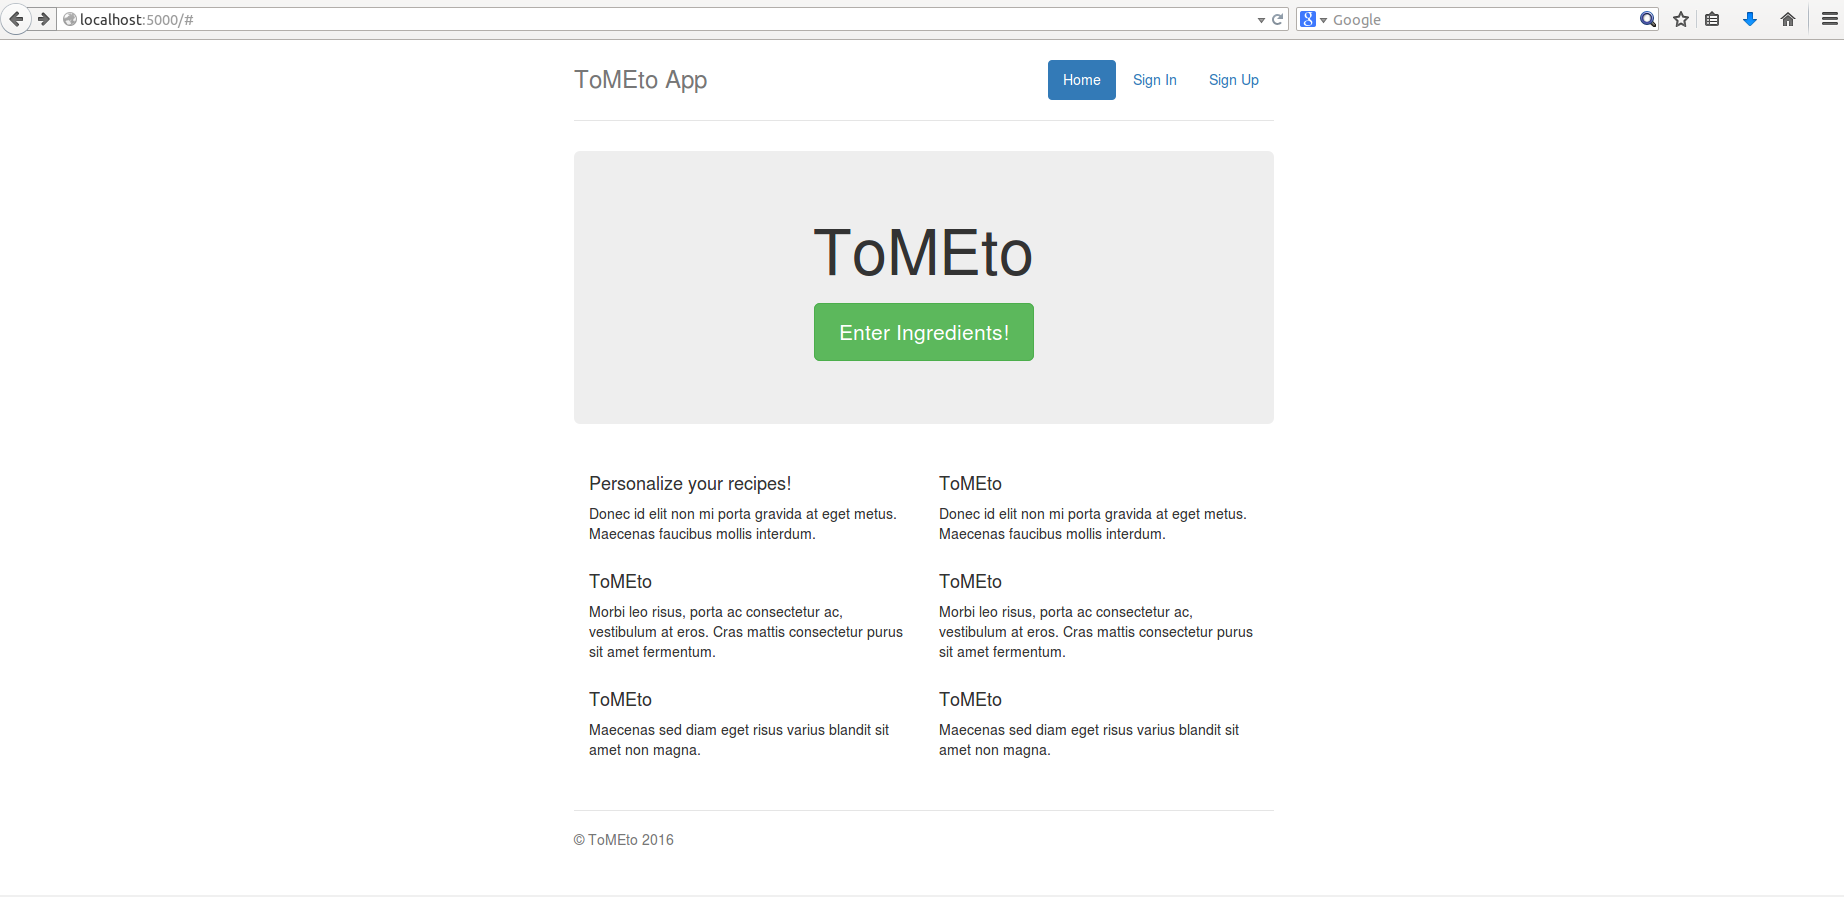
\includegraphics[scale=0.3]{firstpage.PNG}
\end{center}

And our submission page: \\
\begin{center}
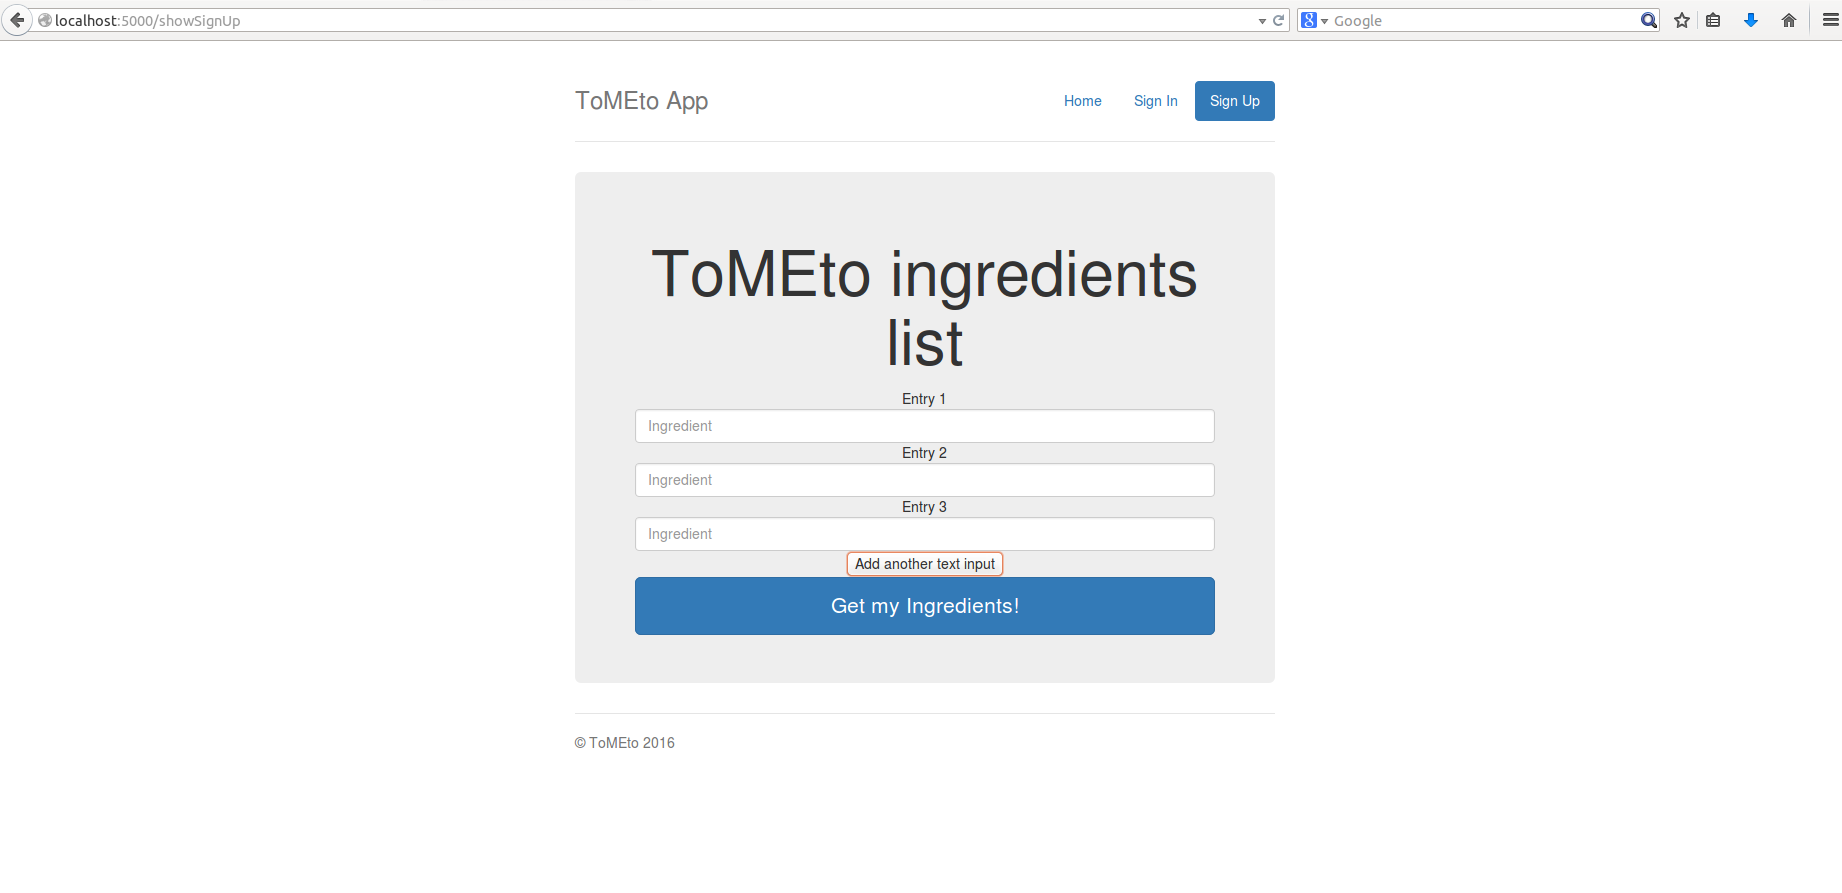
\includegraphics[scale=0.3]{secondpage.PNG}
\end{center}
 

The major challenge was learning about front-end development. Furthermore, while there existed sites which explained the implementation of certain features, it was difficult to determine how the existing code worked, and modify it as needed. 

This basic layout is useful for testing purposes and offers a good foundation for the further development of our web application. From this, we know that integration of back-end and front-end should not be too much of an issue, as the large part of linking the two was accomplished with our test webpage.

TODO: As far as front-end, there is a lot that can be done to improve the overall look and feel of the webpage. Once we get a better idea of our target use cases, we can edit the formatting and the entry forms on our webpage to be more intuitive regarding the use case, as well as add some descriptions on what ToMEto actually does. 





\end{document}

